
\section{Stata} 
In this section, I go over some basics and tools in Stata. It's really hard to demonstrate interactive software in a PDF file, and I do not attempt to do that. I will go over some key components of the software and dive directly into useful practices, commands, packages, etc. For those who need more navigation as a starter, there are many useful YouTube videos online, which are much more efficient.

\subsection{Elephant in the Room, but Not Really}
\label{sec_elepant}
Let me start with the elephant in the room. The most often complaint I hear people say about Stata is that it can only work with one dataset at a time. This is only 10\% true. You can certainly --- and easily --- work with multiple datasets in Stata, with two sets of commands: \verb|preserve|/\verb|restore| and \verb|tempfile|. We will get to them later in this section. But first, let's see what that 10\%-true is about. 

Stata has a very particular way of handling the datasets you work with. I'd like to imagine Stata as a desk:
\begin{figure}[H]
    \centering
    \caption{Stata as a Desk}
    \label{fig_desk}
    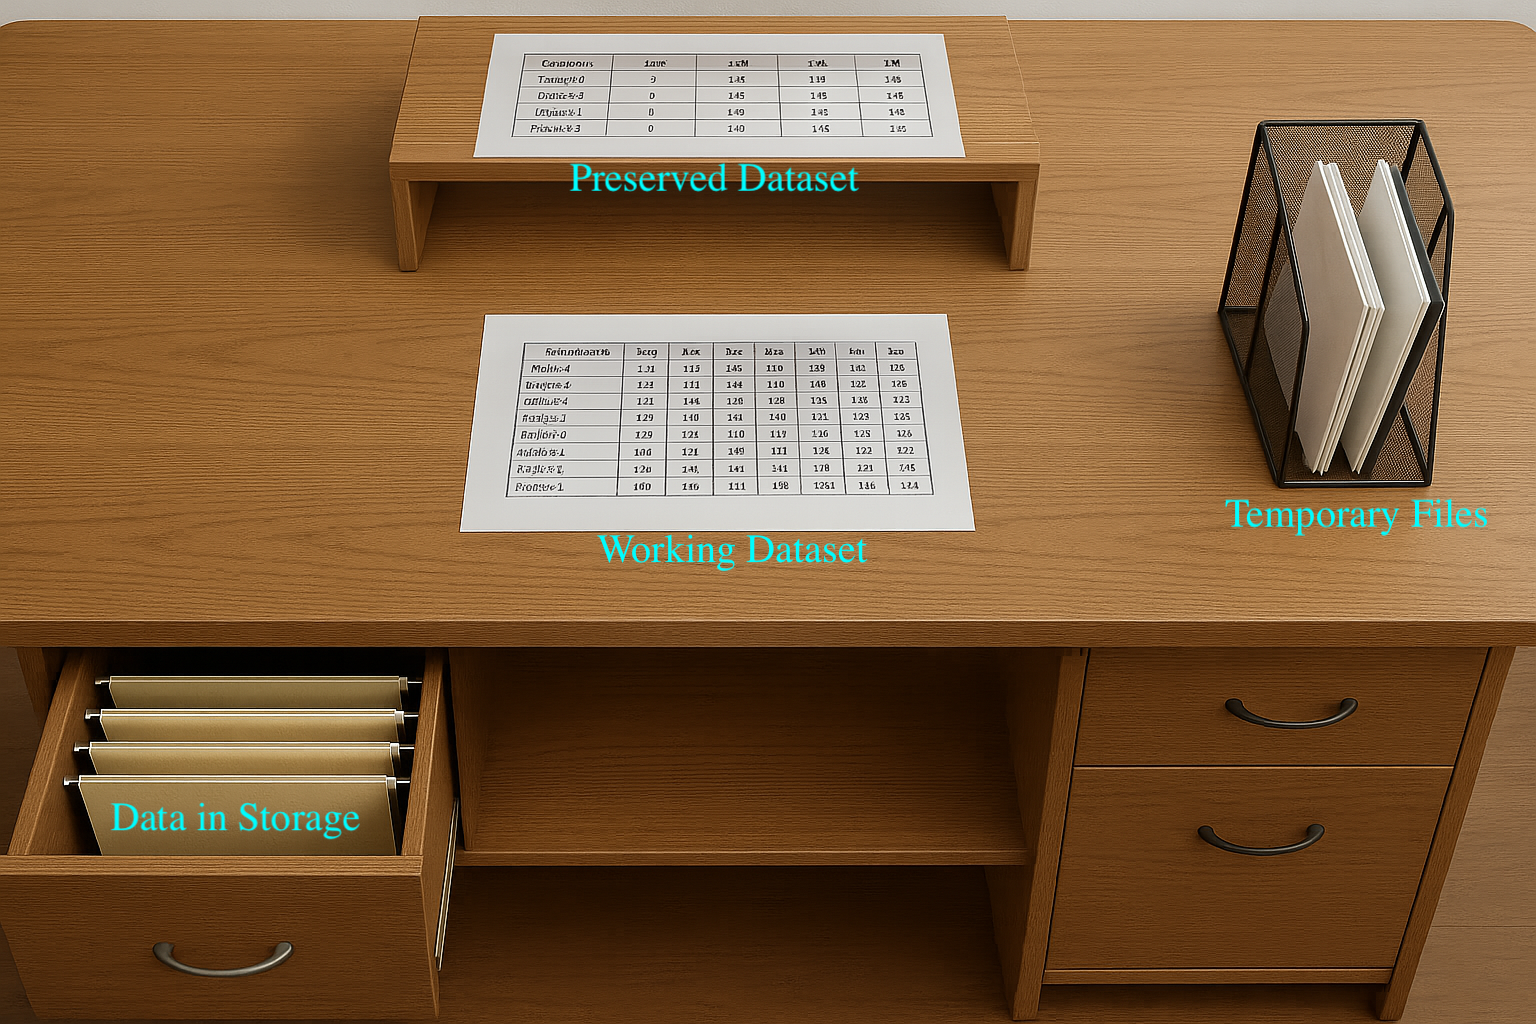
\includegraphics[width=0.9\linewidth]{Output/Figures/desk.png}
    \caption*{\scriptsize\textbf{Note:} Generated by ChatGPT.}
\end{figure}

\paragraph{Working Dataset} In the center of the desk, there is a single dataset that you are currently working on; let's call it the ``working dataset''. This is the data that you are messing with. All your commands for manipulating and analyzing variables operate on this dataset. This working dataset changes and evolves as you run commands. The working dataset is all you can see at any moment. Your eyes are fixed on the center of the desk, and in order to read and modify anything else, you have to pull it to the center of the desk. Your desk is small, so there can only be one working dataset at a time. 

\paragraph{Preserved Dataset} At the top of the desk, there is a little shelf (or a monitor stand that doesn't have a monitor on it). This is like a back pocket where you can hold a copy of the status quo of your working dataset. Let's call it the ``preserved dataset''. Any time you run the command ``\verb|preserve|'', you get a copy of your working dataset at this moment and put it on the little shelf. Then, whenever you run ``\verb|restore|'', you pull the dataset on the shelf back to the center of the table, replacing your working dataset. You will see some demos in the code in the companion repository. Notice that there is only one shelf, meaning that at any given moment, there can be only one preserved dataset. You can't overwrite a preserved dataset if there is already one on the shelf. 

\paragraph{Temporary Files} You also have a big magazine rack on the corner of your table, where you can save as many temporary files as you want. You can give them names and overwrite them. It's called temporary because whenever you are done with your work (e.g., closing Stata), your room service comes in and clears everything on the table: the working dataset, the little shelf, and the magazine rack. 

\paragraph{Data in Storage} In the end, you have your desk drawers, where you have all your datasets saved in your computer's storage. Of course, you can load data from there anytime you want, and save, modify, replace, or delete anything from there. 

We will go through how to use these commands later. But first, let's start with some basics. 

\subsection{Windows}
\begin{figure}[H]
    \centering
    \caption{Three Main Windows}
    % \label{fig:enter-label}
    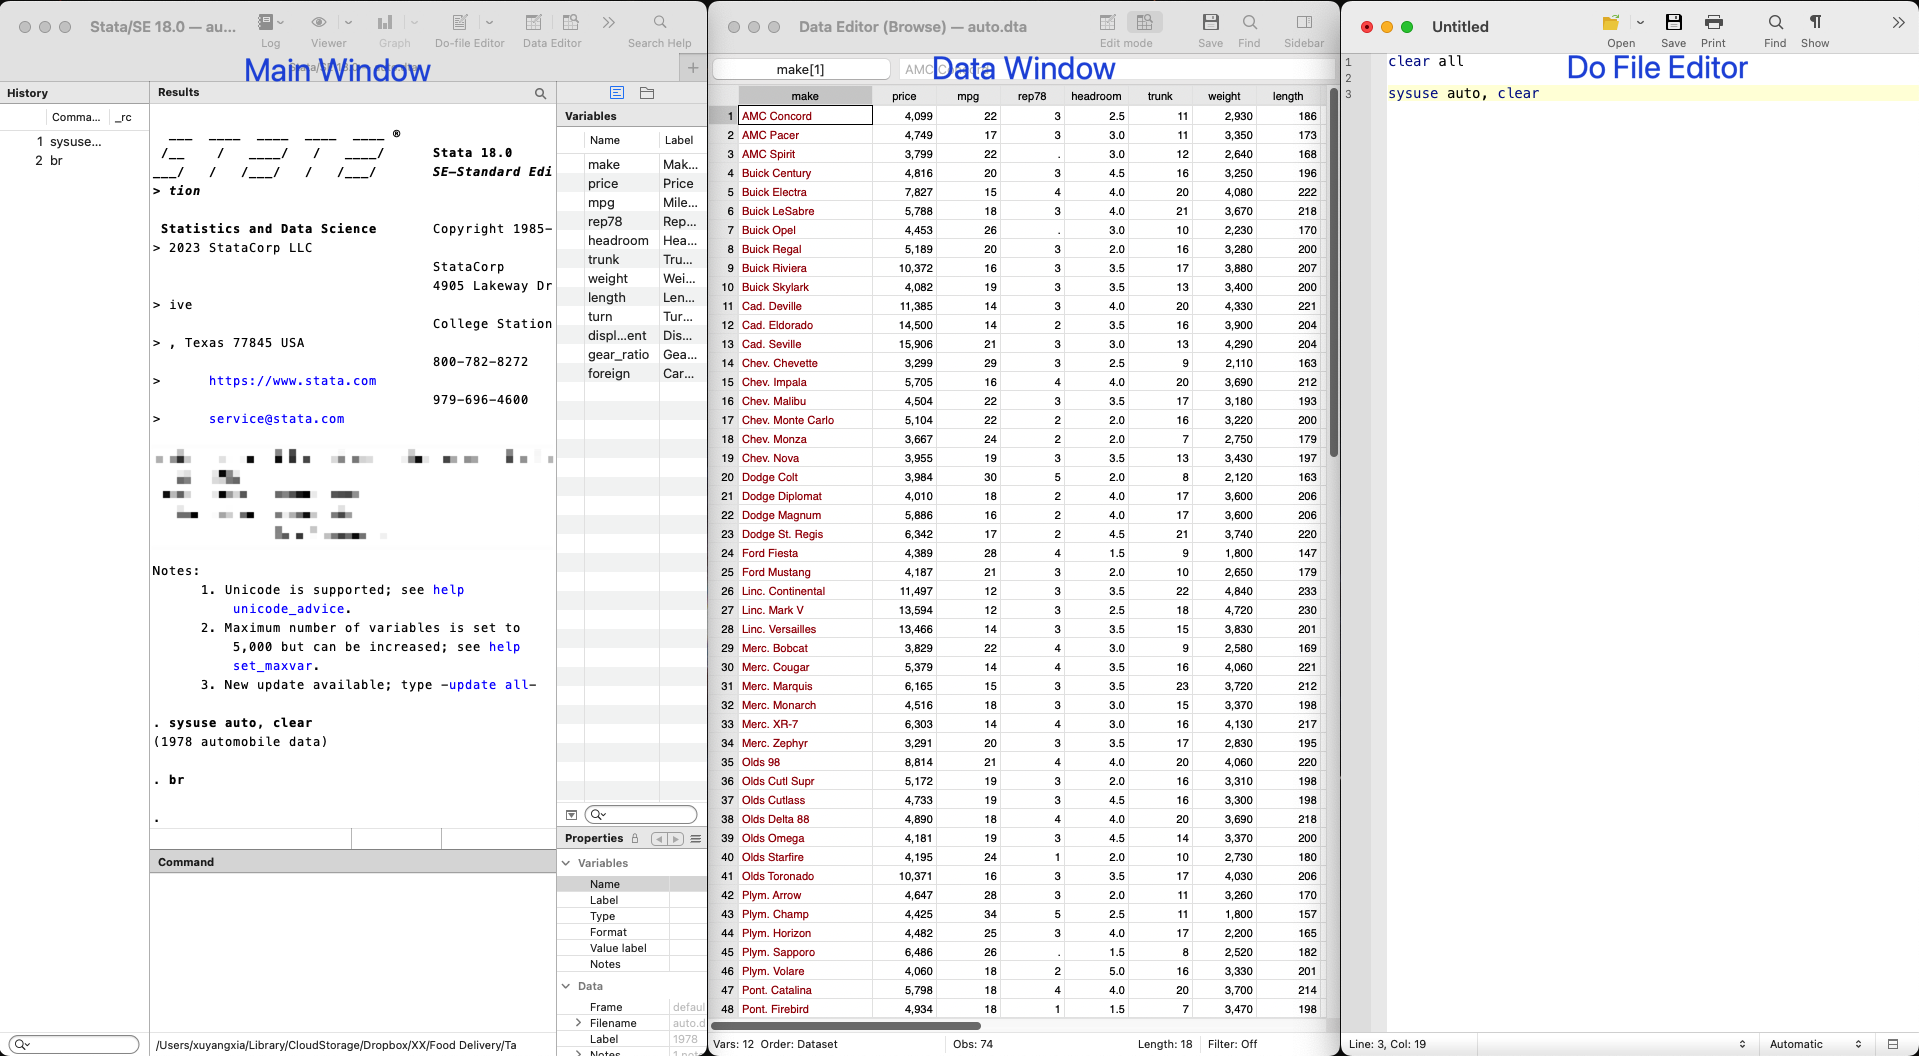
\includegraphics[width=\linewidth]{Output/Figures/windows.png}
    % \caption*{\scriptsize\textbf{Note:}}
\end{figure}
Most of the time, you will be mainly interacting with three windows:
\begin{itemize}
    \item Main Window (left): This is where most things happen. It consists of multiple tabs:
    \begin{itemize}
        \item \verb|Command|: You can type any command directly into here, and press Enter to run it. This is mainly for you to try some quick analysis or navigate the datasets, without saving them into a script.
        \item \verb|Results|: Shows the results of your command.
        \item \verb|History|: Records all commands you have run.
        \item \verb|Variables|: Shows all the variable names and labels.
        \item \verb|Properties|: Shows the details of the data (size, etc.), and if you select one variable from \verb|Variables|, it will also show the details of that variable here, like its type, format, etc.   
    \end{itemize}
    \item Data Window (middle): This window shows your data. It shows up when you run \verb|br| command, or click the top icon in the main window with a magnifier. You can search for stuff here (\verb|Ctrl/Cmd+F|) or open the side bar at the upper-right corner to select variables to view, etc. 
    \item Do File Editor (right): This is where you write, run, and save your script.  
\end{itemize}

\subsection{Run Commands in Do File Editor}
\label{sec_run_commands}
\begin{figure}[H]
    \centering
    \caption{Two ways}
    % \label{fig:enter-label}
    \subfigure[Do]{
\includegraphics[width=0.2\textwidth]{Output/Figures/do_icon.png}}\hspace{3cm}
    \subfigure[Execute (include)]{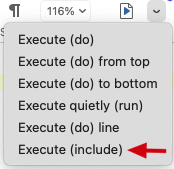
\includegraphics[width=0.2\textwidth]{Output/Figures/include.png}}
    % \caption*{\scriptsize\textbf{Note:}}
\end{figure}
There are multiple ways to run code in a script.
\begin{itemize}
    \item If you don't highlight anything and click the \verb|Do| icon at the upper-right corner, it will run the whole script. 
    \item If you highlight something and click the \verb|Do| icon at the top, it will run the highlighted part. 
    \item If you highlight something and click \verb|Execute (include)| under the arrow next to the \verb|Do| icon, it will run the highlighted part as if you paste it into the Command tab in the main window and then run it. 
\end{itemize}
\verb|Execute (include)| can be very useful. If you run via \verb|Do|, even just a part of the code, when the execution is completed, it does two things automatically: i) forgets all local macro names (What are these? We will talk about them later); ii)  replaces the working dataset with preserved dataset (if there is any). Sometimes, when we test the code and run it line by line, we may not want these things to happen, which is when we run it via \verb|Execute (include)| instead. 

\subsection{Things Skipped in This PDF and Some Quick Notes}
I won't be able to cover all the details in this PDF, so I will selectively skip explaining some stuff. I will introduce you to some basic commands to get you started. With the understanding of the syntax and basic commands, you can easily figure out how other commands or packages work, which will not be covered in detail in this PDF. I will then cover some quasi-fancy stuff in writing programs and packages, whose syntax is somewhat special. I will skip some extra fancy/nerdy stuff that is mostly for things Stata \textit{can} do, but you may want to use something else if you can for your own sanity. 

The dataset Stata processes has the standard data table format: each row is an observation, and each column is a variable. Manipulating data with other layouts, such as matrices, can be a little tricky. It's not impossible, but it's not what Stata is designed for. So if you have to deal with lots of matrix calculations and manipulations, tools like MATLAB or Julia may be much better choices. 

Many Stata command comes with a shorter abbreviation, which is always the first few letters of the original command. For example, \verb|br| does the same thing as \verb|browse|, \verb|reg| for \verb|regress|, \verb|di| for \verb|display|, etc. In this document, I use the abbreviations most of the time, especially for commonly used commands, so you can get used to them and save some typing in your own scripts. If you see a command elsewhere that doesn't look the same as I put in this file, check if it's just an abbreviation. Many commands do not have abbreviations, most of the time intentionally. For example, commands for modifying or deleting information from the data often do not have abbreviations --- \verb|drop|,  \verb|collapse|, etc. --- just so you don't do it by accident.  

\subsection{Basic Commands}
\label{sec_basic_commands}
In this section, I go through some basic and important Stata commands. The most common structure of a Stata command is 
\begin{verbatim}
   [command name] [variable/dataset name(s)] [if condition] [,] [options] 
\end{verbatim}
For example, 
\begin{verbatim}
   reg y x if year>2005, r
\end{verbatim}
uses the command named \verb|reg| to run an OLS regression with dependent variable \verb|y| and independent variable \verb|x|, using observations whose \verb|year| is larger than 2005, and the option \verb|r| asks the program to produce the robust standard errors. 

Notice that most commands only have one comma, which separates the main command and its options. This implies that Stata uses spaces, instead of commas, to divide objects in the command. 

Stata has very good documentation for its commands. If you want to learn more about a command, just type \verb|help [command name]| in the Command tab in the main window, and then you can see the documentation of that command. Or you can just Google ``Stata \verb|[command name]|'' and chances are the official documentation will show up at the top. It's highly recommended to spend some time reading some of these documents, because most of them follow a very standard format, and after reading a few, you will figure out the pattern and where to find the stuff you need. 

In the rest of this subsection, I will go over some commands, highlighting the most important stuff. I will not go through every single detail of each command, so if you want to learn more or have questions regarding some specific use cases shown in the code, try reading the documentation or asking ChatGPT.

\paragraph{\underline{use}} This command loads data as the working dataset. One thing to notice is that if the data you want to read is too large, you may selectively load part of the dataset, like some specific variables or observations that meet certain criteria, to speed things up. For example, 
\begin{verbatim}
    use year age brand* income*_adj using "data_file.dta" if year>2005, clear 
\end{verbatim}
reads variables \verb|year|, \verb|age|, all variables whose name start with \verb|brand|, and all variables whose name start with \verb|income| and end with \verb|_adj|, from the dataset \verb|"data_file.dta"|, only for observations whose \verb|year| is larger than 2005, and the option \verb|clear| tells Stata to overwrite the current working dataset if there is anything already loaded. 

Notice that here we use \verb|*| to indicate a group of variables that share the same pattern in their name. This is called ``wildcard'' and is very useful. We will use this very often in the code. 

If you want to load all variables of a subsample, you can do 
\begin{verbatim}
    use * using "data_file.dta" if year>2005, clear 
\end{verbatim}
And if you just want to load the whole dataset, just do
\begin{verbatim}
    use "data_file.dta", clear
\end{verbatim}

The quotation marks on the dataset are not required, but I like to use them since they will make the dataset name show in a different color, so it's easier to tell it's a dataset. Also, if your file path has spaces in it, you have to add the quotation marks. More details are here: \url{https://www.stata.com/manuals/duse.pdf}

Here should also be the place where I demonstrate how to load data in other formats: Excel, CSV, SAS, etc. But honestly, I never memorized how to do them. There is a simple way to figure out the syntax. In your main window, click \verb|File| at the upper left, then \verb|Import|. There you can find interactive windows to load many data formats. Once you are done specifying the settings in the window, you can see a command shown in the Results tab that corresponds to the settings you just specified. Copy that into your do file, then you are pretty much done. You can make adjustments on it as needed, e.g., changing the file/path name, adding \verb|clear| option, etc. By doing so, you don't have to memorize the syntax for importing each data format. Similar ways work for exporting files when you want to save your working data into a different data format. 

\paragraph{\underline{keep} and  \underline{drop}} They can be used to keep/drop variables, as well as observations, depending on how you write the commands. If it's followed by variable names, it keeps/drops the variables. For example, \verb|keep v1 v2 x*| drop all variables in the working dataset except for variables \verb|v1|, \verb|v2|, and all variables whose name starts with \verb|x|. On the flip side, \verb|drop v1 v2 x*| drops these variables from the data set. 

If the command is followed by a \verb|if| condition, then Stata would understand it as keep/drop observations. For example, \verb|keep if year>2005| only keeps observations in the working dataset whose \verb|year| is larger than 2005. 

You can also do math or use multiple variables in the \verb|if| condition. For instance, 
\begin{verbatim}
    drop if x==y*2
\end{verbatim}
drops observations whose variable \verb|x| is equal to two times its variable \verb|y|. Notice that once a symbol like \verb|*| is not used in variable names, Stata interprets it as the common mathematical operations, instead of a wildcard as we used above. 

You can also use logical operators such as ``and'' (\verb|&|), ``or'' (\verb|||), ``not'' (\verb|!|), etc. in the \verb|if| condition. Different parts of the condition can be separated by \verb|()|. Check out details here: \url{https://www.stata.com/manuals13/m-2op_logical.pdf}.
\paragraph{\underline{br}} This command allows you to open the data window and see the status quo of your working dataset. You can also specify what variables and what observations you want to see. \verb|br v1| only shows you the variable \verb|v1|; \verb|br if year>2005| shows you all variables but only for observations whose \verb|year| is after 2005; and \verb|br v1 if year>2005| only shows \verb|v1| for this subsample. 

This seems like a very simple command, but I personally find the ease of navigating data in Stata underrated. It's very helpful to have a direct view of what you are working with, and since the data window updates itself every time you run a command, you can also track if the dataset changes in a way that you expect it to. This is one of the main reasons why I feel more confident using Stata to clean the data. You can just directly type in the command window whatever you want to see, without worrying about generating new datasets or variables.  

\paragraph{Commands for Quick Summary Stats} You can easily check the summary stats of your datasets and variables at any given point. Here are a few commands that you will use all the time.

\verb|su| gives you some simple summary stats of all the variables in the working dataset. You can also do \verb|su v1 v2| to just check a few variables, and \verb|su v1,de| for more detailed summary stats including percentiles. It also saves all the summary stats into some local scalars (more on this below) that you can access after running the command. Simply type \verb|return list| to check what statistics are saved. 

\verb|tab| gives you the frequency of each category in a categorical variable. \verb|tab v1| shows the details of \verb|v1|, and \verb|tab v1 v2| shows a two-way tabulation of two categorical variables. You can also add options like \verb|row| or \verb|cell| to get the percentage of each category. See more details here: \url{https://www.stata.com/manuals/rtabulateoneway.pdf} \\
and \url{https://www.stata.com/manuals13/rtabulatetwoway.pdf}. If your variable has too many categories, then \verb|tab| would refuse to work. In that case, the package \verb|fre| can be used; see \url{http://fmwww.bc.edu/repec/bocode/f/fre.html}

\paragraph{\underline{gen}} This command generates new variables, and is probably the one that you will use the most. \verb|gen v3 = v1+v2| generates a new variable \verb|v3| that is the sum of the existing variables \verb|v1| and \verb|v2|. But there are a lot more things you can do with it. Check out the code in the companion repository and the help file \url{https://www.stata.com/manuals/dgenerate.pdf}. 

One thing to note here is variable types. Stata has multiple variable types for numbers and strings. This is not something you need to worry about most of the time, since Stata automatically detects the variable type when generating it, and updates the type when needed. But there are some special occasions when you may want to specify the variable type. There is an example in the companion code \verb|01_data_cleaning_and_manipulation|.

\paragraph{\underline{egen}} This is \verb|gen| on steriods. It comes with all kinds of functions that allow you to do all kinds of things. Make sure to check out the help file: \url{https://www.stata.com/manuals/degen.pdf}. One common use case is to generate summary variables while maintaining the data structure. For example, \verb|egen v3 = total(v1)| generates a variable that is the sum of \verb|v1| across all observations, and most importantly, it does so by adding \verb|v3| to the working dataset where every observation has the same value of \verb|v3|. If it's not clear what this means to you, just try it out. Combined with the \verb|bys| command below, it can also easily generate summary variables by groups. 

\paragraph{\underline{bys}} This is the abbreviation of \verb|bysort|. It does two things. First, it sorts the data as instructed; second, it tells Stata to perform the command that follows \textit{by groups}. For example, in the working data, each observation is a person with her unique \verb|id|. Each observation works for a \verb|company| with an \verb|income|. Then 
\begin{verbatim}
    bys company: egen inc_comp = total(income)
\end{verbatim}
calculates the total income in each company, and all observations that belong to the same company would have the same value on the new variable \verb|inc_comp| that is the total income of that company. This line of code above is equivalent to 
\begin{verbatim}
    sort company
    by company: egen inc_comp = total(income)
\end{verbatim}
which sorts and generates the new variable in two separate steps. You can't use \verb|by| if the data is not sorted by the variable that you use to define the groups, but once it's sorted, you can perform multiple \verb|by| commands using the same groups. 

You can also do \verb|bys v1 (v2 v3): egen ...|. This tells Stata to sort the dataset by \verb|v1|, \verb|v12|, and \verb|v3|, and then conduct the calculation by groups defined by \verb|v1|. This operates the same as 
\begin{verbatim}
    sort v1 v2 v3
    by v1: egen inc_comp = total(income)
\end{verbatim}
This is very useful, especially when combined with \verb|_n| as shown below. 

Notice that \verb|sort| only sorts variables in a descending order. If you want to sort in ascending order, use \verb|gsort|. E.g., 
\begin{verbatim}
    gsort v1 -v2 -v3
\end{verbatim}
first sorts observations by descending order of \verb|v1|, then ascending order of \verb|v2| and then \verb|v3|.

It's worth noting that \verb|gen| also comes with a \verb|sum()| function. However, it calculates the \textit{cumulative} sum within the group, instead of the total sum. E.g., 
\begin{verbatim}
    bys company (age): gen inc_cumu = sum(income)
\end{verbatim}
generates a variable that, within each group, the first observation's \verb|inc_cumu| is its own income; the second observation's \verb|inc_cumu| is its own income plus the first observation's income; the third observation's \verb|inc_cumu| is the sum of the first, second, and the third, and so on. This may seem a strange function, but it can actually be very useful and used creatively for different purposes, especially when used with panel data. You will find some examples in the companion code. 

\paragraph{\underline{\_n} and \underline{\_N}} These are not commands per se, but very useful system variables --- variables that are automatically generated in the background. \verb|_n| indicates the index of each observation based on the current sorting, so the first observation has \verb|_n=1|, the second \verb|_n=2|, and so on. \verb|_N| is the index of the last observation. 

They are often used with \verb|[]| after a variable, which refers to the value of the variable for a specific observation. For example, \verb|v1[1]| indicates the value of \verb|v1| for the first observation and \verb|v1[_N]| indicates the last. If you do \verb|gen v2=v1[_n-1]|, then \verb|v2| will be a new variable that takes the value of \verb|v1| from the previous observation. \verb|v2| will have missing for the first observation, because there is no observation before it.  

They are often used with \verb|bys|, where if you use \verb|_n| or \verb|_N| behind a \verb|bys|, they refer to indices within each group. For example, \verb|bys group (age): gen v3=v1[1]| generates a new variable \verb|v3| that is the value of \verb|v1| for the first observation within each group; in this case, \verb|v1| for the youngest person within each group. Similarly, \verb|v3| will be missing for the first observation in each group. 

\paragraph{\underline{collapse}} All the commands mentioned above maintain the level of observation in the data; e.g., if your dataset is at the individual level, then after applying the commands above, each observation remains an individual. \verb|collapse| literally collapses the dataset to a higher level / by groups. For example, suppose your working dataset is currently at the individual level, with each observation having a unique \verb|id|, then 
\begin{verbatim}
    collapse (mean) age (max) height (count) id, by(group)
\end{verbatim}
gives you a new dataset that has four variables. Each observation now is a group, with its identifier \verb|group|. And in the new dataset, \verb|age| is the mean of the age of all individuals in the group; \verb|height| is the maximum height in that group, and \verb|id| is the number of individuals in that group. Keeping the original variable names is confusing, which is why you can also customize the names of the collapsed variables, and also collapse different statistics for the same variable, for example, 
\begin{verbatim}
    collapse (mean) mean_age=age (max) max_age=age max_height=height 
\end{verbatim}
\begin{verbatim}
             (count) N=id, by(group)
\end{verbatim}
As you can already tell, stuff in \verb|()| indicates the type of statistics to calculate; there are many types of statistics you can do, which can be found here: \url{https://www.stata.com/manuals/dcollapse.pdf}. The stuff before \verb|=| is the name of the new variable, and the stuff after \verb|=| is an existing variable in the current working dataset. Stuff in \verb|by()| indicates the group, which can also be defined by multiple variables, e.g., \verb|by(group gender)| will collapse the dataset to each group-gender category. 

Another technical note. When you run \verb|collapse|, Stata first saves a copy of the working dataset and then does the collapsing. In case anything goes wrong, it will report an error and retrieve the original dataset, so you can fix the bug and run it again. When your dataset is large, however, saving a copy and be very time-consuming. In this case, you may add the option \verb|fast| after the comma. This tells Stata to skip saving the copy and collapse right away. The tradeoff, of course, is that if there is any error during collapsing, you will have to regenerate the pre-collapse dataset again. 

\paragraph{\underline{assert}} This is my favorite command in Stata, and it does nothing to the dataset. Instead, you can put whatever statement behind this command, and it will output an error if the statement is wrong. This is extremely useful for checking your code. At any point in the code, you can come up with any sanity checks --- i.e., any conditions that you think the current dataset should satisfy ---and then insert an \verb|assert| command to check if it's correct. 

It can be used during the process of writing the code, and you can also leave it in the code for future checks. For example, you may have many \verb|assert| statements in your script; when you later run the script again, if the statement is correct, then it does nothing and the code proceeds; if the statement is wrong, then it will report an error and the code will stop. So, e.g., if the dataset is slightly changed and you need to run the script again, it can help you make sure if the code still makes sense. 

It can process statements on scalars, e.g., \verb|assert 4==2^2| or checking if the mean of the variable \verb|v1| is below 1:
\begin{verbatim}
    su v1
    assert `r(mean)'<1
\end{verbatim}
I also sometimes do 
\begin{verbatim}
    unique id 
    assert `r(unique)'==`r(N)'
\end{verbatim}
to make sure each observation in the data is a unique \verb|id|. The command \verb|isid| does very similar things, but differs slightly in dealing with missing values, and \verb|isid| also automatically sorts the data. 

\verb|assert| can also process observation-wise checks --- a statement on each observation --- and it will report an error unless all observations satisfy that statement. For example, \verb|assert v1<1| asserts that \verb|v1| is smaller than 1 for all observations. 

You can be creative in the statement to test. But remember, it will stop the code if the statement is wrong. So if you are running a long code, just make sure the assertions are necessary. 

\paragraph{\underline{merge}} This command merges the working dataset with another dataset. You will have to specify one or multiple variables as the key to merge, and it can be a one-to-one merge (\verb|1:1|), multiple-to-one merge (\verb|m:1|), or one-to-multiple merge (\verb|1:m|). The syntax is very straightforward
\begin{verbatim}
    merge 1:m key1 key2 using "dataset_2.dta"
\end{verbatim}
After running it, it will show you a summary stats the merge: how many observations are merged, and how many are not merged in the master dataset (i.e., the working dataset) and the using dataset. It also generates a new variable \verb|_merge| that specifies the category of each observation (1 for not merged in master; 2 for not merged in using; 3 for merged). 

\verb|merge| also has a \verb|assert()| option. For example, if you think all the observations in the working dataset should be matched, then you can do 
\begin{verbatim}
    merge 1:m key1 key2 using "dataset_2.dta", assert(2 3)
\end{verbatim}
In this case, if Stata finds any observations in the master data that are not matched with any observations in the using data, it will report an error and stop. This helps you check problems in the code. 

You can also specify what categories to keep using option \verb|keep()|, and tell Stata not to generate \verb|_merge| by adding \verb|nogen| option. However, if you have, say \verb|keep(1 3)|, the output window will not show how many observations in the using data that are not matched (it will just say 0 observations in category 2), which may mask some problems. Therefore, \verb|keep()| and \verb|nogen| are not recommended unless you are certain what you are doing, and ideally accompany it with the \verb|assert()| option. 

If the master and the using datasets have variables that are not key but have the same name, the default would keep the variable from the master dataset. You can instead tell Stata to \verb|update| or \verb|replace|. See more details here: \url{https://www.stata.com/manuals/dmerge.pdf}.

Another important note: \textbf{DO NOT USE} \verb|m:m|. It does not do what you think it does, and is not recommended for use in any scenario. If you want to perform a multiple-to-multiple merge and create observations for all pairwise combinations of the key, use \verb|joinby| instead. Its syntax is very similar to \verb|merge|. More details here: \url{https://www.stata.com/manuals/djoinby.pdf}.

\subsection{Macro Names} This is the most exciting and somewhat unique (at least in its ease of use) feature in Stata, and can offer substantial flexibility and possibilities to the things you can do. The most often used macro names are global and local names for strings. They work in similar ways, so I will use local names as the example and explain global names later. 

Think of a local name as an object that you can assign any string to, and then later you can insert that string back into your script by referring to the name. For example,
\begin{verbatim}
    loc mylocal1 = "*v2"
    gen v3 = v1`mylocal1'
\end{verbatim}
In the first line, we create a local name called \verb|mylocal1| and assign it with the string \verb|*v2|. In the second line, we plug the local name back into our script by putting the name between \verb|`| (the key to the left of 1 on your keyboard) and \verb|'| (the single quote). What Stata does is to read \verb|`mylocal1'| as whatever string you assigned to it; in this case, it reads \verb|`mylocal1'| as \verb|*v2| (without the quotation mark), and therefore treats the second command as \verb|gen v3 = v1*v2|. 

The usage of the local name above is just for illustration purposes and is not necessary at all. But hope you've got the idea of how it works. Notice that Stata reads local names quite literally; it just runs whatever the code would be once the local names are plugged in. This means you can write code with code. We will see some examples in the next section with loops. 

Local names are automatically overwritten if the same name is assigned a different value. If a local name is used but not initialized and assigned any value beforehand, there will be \textit{no} error; instead, Stata would just read it as an empty string. 

Another common use case of the local names is to allow you to change many places in the script all at once. The best example is file paths. Suppose you save all your data files into the folder \verb|C:/folder_1|. Then, for some reason, you move them to a different folder, or someone else wants to run your code, but they save their data files under the folder \verb|Dropbox/folder_A|. In this case, when you write the code, you can leave flexibility in the file path by defining a local name at the beginning of the script
\begin{verbatim}
    loc datapath "C:/folder_1"
    use "`datapath'/my_data1.dta", clear 
    merge 1:1 id using "`datapath'/my_data2.dta"
    ... 
\end{verbatim}
And you use the local name instead of the real path everywhere in the script. Then, when the file location is changed, one just needs to simply change the string assigned to the local name at the beginning, and everywhere else will be taken care of automatically.

Global names work basically the same way as local names, except that they are "global", meaning Stata will remember them all the time, in any scripts, until Stata is closed. To define them, use \verb|gl|, and to use them, type \verb|$| or \verb|${}|. Here is an example using global to define the file path, which is what we usually do when the file path applies to multiple scripts, or when you want some names to be used inside some programs (more on this later). 
\begin{verbatim}
    gl datapath "C:/folder_1"
    use "${datapath}/my_data1.dta", clear 
    merge 1:1 id using "${datapath}/my_data2.dta"
    ... 
\end{verbatim}

You may wonder what if you want your string to have \verb|""| in it. In this case, you will need to use a "bigger" quotes, \verb|`" "'|, when writing the string. Here is an example:
\begin{verbatim}
    gen v1 = 1 // Create a variable that is 1 for all observations.
    loc mystr = "v1"
    gen v2 = `mystr' // This generates a new variable v2 that is the same
                         as v1, i.e., also 1 for all observations.
    loc mystr = `""v1""'
    gen v3 = `mystr' // Stata reads this line as gen v3 = "v1", therefore
                        it generates a string variable v3 that takes the 
                        value of the string "v1" for all observations. 
\end{verbatim}
Since local and global names literally become part of the script, you may find yourself coming up with all kinds of creative ways to use them. Some examples in the later sections and in the repository may give you some inspiration. 

\subsection{Loops}
In this section, we talk about how to write loops in Stata. Here should also be the place where I mention how to write if statements, but I will skip that, since it's very straightforward and I am sure you can easily figure it out yourself by Googling it or reading the code in the repository. 

There are three main ways to write loops, depending on your needs. The basic principle is the same: you define an object with a name, and let it take a series of values. In Stata, this object is treated as a local string name as introduced in the previous section, and inside the loop, you just refer to the object by putting its name in \verb|`'|.

\paragraph{Simple loop on any local strings}
Since the object to be looped on is a local name, it will become part of the code inside the loop, so basically you can assign it anything
\begin{verbatim}
    foreach i in Stata is pretty good {
        di "`i'" // "di" is for printing stuff in the Results window.
    }
\end{verbatim}
And in the Results window, you will see
\begin{verbatim}
    Stata
    is 
    pretty 
    good
\end{verbatim}
If you don't add quotation marks, Stata will divide each value by spaces. Or you can do 
\begin{verbatim}
    foreach i in "Stata is" "pretty good" {
        di "`i'" 
    }
\end{verbatim}
and Stata will treat each quote as a single object and print
\begin{verbatim}
    Stata is 
    pretty good
\end{verbatim}
Of course, you can also loop over numbers, variable names, etc. as you like.

\paragraph{Loop over variables}
This is for looping over a bunch of variables. The main reason you want to use this is to leverage wildcards for referring to variables. For example, you want to generate a squared variable for every existing variable whose name starts with \verb|v| or \verb|haha|:
\begin{verbatim}
    foreach i of varlist v* haha* {
        gen `i'_squared = `i'^2
    }
\end{verbatim}
And that's it. 

\paragraph{Loop over many scalars}
Commonly, one may want to loop over an array of values, say from 1 to 10, in which case you can use 
\begin{verbatim}
    forval i = 1/10 {
        di `i'
    }
\end{verbatim}
You can also specify the step size or do it in a decreasing order
\begin{verbatim}
    forval i = 50(-2)0 {
        di `i'
    }
\end{verbatim}
More usage can be found here: \url{https://www.stata.com/manuals13/pforvalues.pdf}.

\paragraph{\underline{levelsof}} This command is followed by a categorical variable, and saves the unique values of the categorical variable into a sorted list, which can then be referred to as \verb|`r(levels)'|. One can use this list as an input in a loop, e.g., to loop over all distinct values in the categorical variable. See: \url{https://www.stata.com/manuals/plevelsof.pdf}.

To be honest, for whatever reason, I don't find myself using this command as often as I saw in some other people's code. My hypothesis is that people who are more familiar with languages like R, Python, or Julia would find this command handy, since it's akin to the coding logic of having an array of, say, types, and then you loop over the types to conduct certain procedures. In many cases, there may be a \textit{more Stata} way to achieve the same purposes, e.g., using \verb|egen|, \verb|bys|, etc. It's not certain which way is more efficient in Stata. Generally, you want to avoid too many loops, unless the data is too large and you want to conduct some calculations piece by piece to save some memory space. 

\paragraph{Example: Use code to write code}
Here is an example of how to leverage local names and loops to make your life much easier. Suppose you want to collapse an individual-level dataset to the group level, and you want to calculate the mean, standard deviation, median, and IQR for all variables whose names start with \verb|v|. Instead of typing them all out, you can do
\begin{verbatim}
    loc collinput = ""
    loc statlist = "mean sd p50 p25 p75"
    foreach v of varlist v* {
        foreach stat in `statlist' {
            loc collinput = "`collinput' (`stat') `v'_`stat' = `v' "
        }
    }
    collapse `collinput', by(group)
\end{verbatim}
Here, I use loops to write part of the command in \verb|collapse| into the local string name \verb|collinput|, and then insert it into the actual collapse command. This code also allows me to flexibly change the summary statistics I want by changing the value of the local name \verb|statlist|. This example will help you master both loops and local names, so please spend a few minutes to figure out exactly how and why this code works. A hint: in the collapsed data, the mean of variable \verb|v1| is called \verb|v1_mean|, the median is called \verb|v1_p50|, etc. 

Once you get used to this use case, I’m confident you’ll appreciate how powerful it is. The fact that Stata can interpret local macro names directly within the script fundamentally changes how you write code. I often find it frustrating when switching to other languages and realizing I need workarounds to achieve the same functionality.

\subsection{Working with Multiple Datasets}
As mentioned at the beginning of this section, you can easily work with multiple datasets in Stata. 

The basic idea is simple. You can only mess with one dataset at a time, which is the working dataset. Going back to the desk in \Cref{fig_desk}, at any given time, you can only see and work with the one dataset sitting in front of you; every time you want to look at something else, you have to put the current working dataset aside and pull another dataset to your working space. The methods introduced below are essentially different ways to put the working dataset aside. 

Perhaps the only practical constraint this adds is when you want to open two datasets and look at them side by side. If you really have to do this, you can either open the other dataset directly (e.g., if it's an Excel or CSV file), or open another Stata session --- on Windows, you can do so by right-clicking the Stata shortcut; on Mac, you can type \verb|open -n -a StataSE| in Terminal. 

\paragraph{\underline{preserve/restore}} This is the little shelf at the top of the desk in \Cref{fig_desk}. See \Cref{sec_elepant} for the description. 

\paragraph{\underline{tempfile}} Here I explain how to use \verb|tempfile| in detail. At any point of the program, you can initiate a temporary file by typing
\begin{verbatim}
    tempfile my_tempfile1 
\end{verbatim}
This command, so far, does nothing to your working dataset. It just creates an empty data file in a temporary file path, so that you can save whatever in it. For example, right after running the command above, you can do 
\begin{verbatim}
    save `my_tempfile1' 
\end{verbatim}
This saves a copy of the working dataset into a temporary file, which is named \verb|`my_tempfile1'| --- notice that the file's actual name, in the temporary file folder, is not \verb|my_tempfile1|, but a random name generated by Stata; you refer to that file name by using the macro name \verb|`my_tempfile1'|. 

You can initiate and save tempfiles at any point in the program, as many as you want. Essentially, you are just saving them into new data files. The only difference is that these tempfiles will be deleted automatically once you finish running the program. 

Some more technical notes regarding tempfiles:

If you initiate a tempfile with the same name as the previous one, the previous file itself is not overwritten, but the macro name is. For example, 
\begin{verbatim}
    tempfile tf1 // Initiate the first file under the temporary path.
    save `tf1'
    ... // Make some changes with the working dataset
    tempfile tf1 // A second file is created under the temporary path,
                    and is linked to the macro name `tf1'
    save `tf1'

    use `tf1', clear // Only loads the second file. The first file loses its
                        macro name reference, so although it still exists in 
                        the temporary path, it cannot be referred to anymore.
\end{verbatim}

When saving tempfiles, as in saving a normal dataset in storage, you can add \verb|replace| option to overwrite the existing file if it already exists. \textit{However, use} \verb|replace| \textit{very carefully with tempfiles.} There is a very specific reason. When using any macro name, if the name is not initiated beforehand, Stata interprets it as empty, instead of an error. As a result, if you somehow misspell the macro name of the tempfile when saving it, and with \verb|replace|, Stata would read it as \verb|save, replace|, and therefore overwrites the working dataset (i.e., the data file you last loaded). For example,
\begin{verbatim}
    use "my_data.dta", clear // Load a data file from storage. 
    drop if year<2005
    tempfile my_tempfile1
    save `my_tmpfile1', replace // Here, the macro name is missing a 
                                   letter e, and Stata would instead 
                                   overwrite "my_data.dta"
\end{verbatim}

There may be cases where you have to use \verb|replace| --- e.g., appending files in a loop --- then just double-check that the name is correctly spelled. Or you can write \verb|confirm file `your_tempfile_name'| to make sure that file exists before \verb|save `your_tempfile_name', replace|; if the name is misspelled here, \verb|confirm file| would report an error. But still, you may only have a typo in the save line, so just be careful.

\subsection{Code Example \#1: Data Cleaning and Manipulation}
Let's take a stock and go to the code 
\begin{verbatim}
    01_data_cleaning_and_manipulation.do
\end{verbatim}
in the companion repository to see how the stuff we've gone through so far works in action. 

\subsection{Other Commands and Packages}
There are all kinds of commands and packages in Stata that you can use for different things, and it's impossible to go through all of them here. Instead, I will give a brief overview of how to install and learn commands in this section, and then mention a few common ones to get you started. 

\paragraph{Install packages} Most commands can be installed via the Boston College Statistical Software Components (SSC) archive. Simply type \verb|ssc install [command name]| in the Command tab in Stata's main window. Some other packages need to be installed via certain websites, where you need to use a \verb|net| command. Usually, to install any package, I'd just try scc first, and if it doesn't work, I would just Google \verb|Stata [command name]|, and chances are there is a webpage for that package, and it will describe how to install it. 99\% of the time, you just need to type something in the Command tab and you are all set. 

\paragraph{Where do my package files go?} Type \verb|sysdir| in Stata's Command tab of the main window, and it will show you all the paths where your Stata program files are saved. All default packages should be saved under the path of \verb|BASE|, and the new packages you installed should automatically go to \verb|PLUS| or \verb|PERSONAL|. So, if you are using a server that doesn't have internet and you have to upload the package files yourself, just put the files in the corresponding folder in \verb|PLUS| or \verb|PERSONAL|, which are usually organized by the initial letter of the package name. If you can't find any of the folders listed by \verb|sysdir|, it's either that the folder hasn't been created yet since that path hasn't been used, or the folder is hidden (in which case, Google to see how to view hidden folders in your OS). 

\paragraph{Learn packages} A great feature about Stata is that most packages come with a standardized help file. For installed packages, type \verb|help [command name]| to pull out its help file (or you can just Google the command and its help file usually comes at the top), where you can usually see a very detailed description of how to use the command: the syntax, all available options, etc. Some also come with an appendix about the economic model at the end (e.g., \verb|clogit|), which is very helpful for learning the model, the MLE expressions, etc. Stata also has an actively maintained online community, which makes it very easy to find stuff you need on Google. STATALIST is a very active online forum specifically for Stata. If you Google any questions regarding Stata, chances are there are some entries from STATALIST where someone asked a similar question. Some Stata specialists are actively maintaining the forum and answering questions. Once you spend enough time on it, you will soon be able to spot the usual suspects who always provide great answers. One of them is Nick Cox. He's everywhere. He's the GOAT. 

\paragraph{AI Tools} Chances are, this section will not age well, but I just want to say a few words on the status quo of the ability of AI tools in helping with Stata. Compared to other languages such as Python or Julia, tools like ChatGPT and Gemini are not as good in Stata. For basic stuff, they are fine, but they would soon start making things up when the task gets a bit complex. So, be careful. They usually make things up with \verb|egen|, where they would come up with some functions that \verb|egen| doesn't support. But overall, they are still very helpful. Just try them out and see if their suggestion works. They are particularly helpful at regular expressions, say, with the command \verb|regexm|, when you need to do some manipulations with string variables. 

\paragraph{Some useful commands and packages} Here is a quick run-through of some packages that are commonly used, or not that common, but I personally found useful. I won't get into too many details here. You can see some of them in action in the companion code in this repository, or find other resources online. 

\paragraph{- Dates} Stata is very good at handling date and time variables. Check out \url{https://www.stata.com/manuals/u25.pdf}. 

\paragraph{- Log files} It's a good practice to save a log file for each code script, so you can check when you last ran the script and what happened back then. You can initialize, modify, and overwrite log files within the script. See: \url{https://www.stata.com/manuals13/u15.pdf}.

\paragraph{- Regular expression} Regular expression is basically a standardized syntax for specifying conditions for a string --- e.g., a string starting with two numbers, followed by three lower-case letters and a comma, ... You can easily use regular expressions in Stata, by, e.g., \verb|regexm|. See \url{https://www.stata.com/support/faqs/data-management/regular-expressions/}

\paragraph{- \underline{strpos()}, \underline{substr()}, and \underline{subinstr()}} \verb|strpos| is a simple command that detects whether a string contains a certain character or substring. It returns the position of the first time that the substring occurs. For example, do \verb|gen v2 = strpos(v1,"og")|, then if an observation's \verb|v1| is \verb|"dog"|, its \verb|v2=2|; if \verb|v1| is \verb|"blog"|, its \verb|v2=3|; and if \verb|v1| is \verb|"dog blog"|, its \verb|v2=2|. If the string doesn't contain the substring, it returns 0. 

It's worth noting that if you put any number into an \verb|if| condition, Stata would treat any non-zero numbers as true, and only 0 as false. So, say you want to drop any observations whose \verb|v1| doesn't contain the substring \verb|"og"|, you can just do 
\begin{verbatim}
    drop if !strpos(v1,"og")
\end{verbatim}

\verb|substr| extracts a substring from a string: \url{https://www.stata.com/manuals/m-5substr.pdf}. \verb|subinstr| replaces a substring with something else: \url{https://www.stata.com/manuals/m-5subinstr.pdf}

\paragraph{- \underline{reghdfe}} This command is for running OLS with lots of FEs. It used to be a user-created package (\url{https://scorreia.com/software/reghdfe/}), but I heard it's incorporated as a base command in Stata 19: \url{https://www.stata.com/new-in-stata/high-dimensional-fixed-effects/}. It takes care of FEs efficiently in a linear model, which is much faster than creating dummies for each FE and then inverting the matrix, etc., as the traditional \verb|reg| command does. One note is to pay attention to its syntax for \verb|predict| post-estimation (i.e., when you want to calculate the predicted value after running a regression). The default option for prediction is \verb|xb|, which does \textit{not} include the values of absorbed FEs. There is a similar command for linear IV regressions, \verb|ivreghdfe|.

\paragraph{- \underline{twoway}} This is a base command for plotting all kinds of figures: lines, scatters, etc. It has many different options and can be very flexible. You can see some examples in the companion codes and in the Exhibits section below. 

\paragraph{- \underline{xtset}} This command tells Stata the panel structure of your dataset, so you can conduct certain manipulations more easily. For example, \verb|xtset id year, yearly| tells Stata that the working dataset is a panel dataset, with each \verb|id| having many years. Then, you can 
\begin{itemize}
    \item Use time series operators: lag (\verb|L.|), lead (\verb|F.|), difference (\verb|D.|), etc. For example, in 
    \begin{verbatim}
        gen v2 = v1*L2.v1
    \end{verbatim}
    \verb|v2| is \verb|v1| of this observation times \verb|v2| from the same \verb|id| from 2 years before. Check out page 4 here for more details: \url{https://www.stata.com/manuals13/tstsset.pdf} --- this is the help file for another command called \verb|tsset|, which is what \verb|xtset| is built upon. 
    \item Explore some panel structure of the data. For example, after \verb|xtset|, you can type \verb|xtdes|, which will tell you the distribution of panel patterns: how many \verb|id|'s have records for every year, how many are missing the first year, etc. \verb|xtpattern, gen(new_variable)| further saves each \verb|id|'s pattern into a string variable. E.g., \verb|"11..111"| means this \verb|id| doesn't have the third and fourth years in the data. You can do many things with this pattern variable. For example, if you only want to keep \verb|id|'s that have records in all years, do 
    \begin{verbatim}
        keep if !strpos(new_variable,".")
    \end{verbatim}
\end{itemize}

\paragraph{- \underline{carryforward}} This allows you to "carry forward" some values from one observation to other observations that have missing values in that variable. It's most commonly used in panel data. E.g., you have monthly data on people's characteristics, and some people's heights are missing in some of the months. If you want, you can use this command to fill in those missing by the closest non-missing cell from a previous month. Here is its help file: \url{http://fmwww.bc.edu/repec/bocode/c/carryforward.hlp}, but the web page is not well-formatted. Just type \verb|help carryforward| in your Stata. A similar command is \verb|tsfill|, which must be used after \verb|xtset|.

\paragraph{- \underline{xtevent}} There are many packages for DiD and event studies, and to be honest, it's very hard to keep myself up-to-date. \verb|xtevent| is my favorite for doing event studies. Check out \url{https://github.com/JMSLab/xtevent} for more details, and also the companion code for some simple demonstrations. 

\paragraph{- \underline{maptile}} This is for drawing maps. Very easy to use. \url{https://michaelstepner.com/maptile/}.

\paragraph{- \underline{texdoc}} This command allows you do write anything from Stata to \LaTeX, especially customized tables. \url{https://repec.sowi.unibe.ch/stata/texdoc/}. It's extremely flexible. Making {\LaTeX} tables becomes so easy once you have this command at hand. You can see some examples in the companion code. 

\paragraph{- \underline{esttab}} This command is also for exporting tables, most importantly, regression tables. Honestly, it's very hard to learn this package simply by reading its documentation, since it's a lot. The easiest way is to check out the companion code and copy the code every time you need to use it. The documentation can help you find some additional options to add if needed. \url{http://repec.org/bocode/e/estout/hlp_esttab.html}. 

\paragraph{- \underline{pdslasso}} This is for the post-double-selection method, some also call it double-machine learning, to select the most effective controls among a kitchen sink of control variables to avoid overfitting. Check out \url{https://statalasso.github.io/docs/pdslasso/}.

\subsection{Local and ado Programs}
Now we move on to a separate subject of writing local and ado programs. Similar to other languages, Stata allows you to write functions that conduct specific tasks with certain input, which you can use repeatedly within or across scripts. They are called "programs" in Stata. 

\subsubsection{Define and use a program: a basic example.} Here is a very simple example of a program: 
\begin{verbatim}
    program add_program 
        syntax, v1(varname) v2(varname) newvar(str) [power(real 2)]

        gen `newvar' = `v1' + `v2'^`power'
    end
\end{verbatim}  
After running this code, nothing would happen except that Stata now knows how this program is defined. Then you may run
\begin{verbatim}
    add_program, v1(income) v2(age) newvar("inc_age_3") power(3) 
\end{verbatim}
which is equivalent to running
\begin{verbatim}
    gen inc_age_3 = income + age^3
\end{verbatim}
Hope you may've already got a feeling of what's going on here. \verb|program add_program| defines a program named \verb|add_program|. The \verb|syntax| line defines the input of the function, where the \verb|()| specifies the input type: the input \verb|v1| and \verb|v2| are a variable names; \verb|newvar| is a string; and \verb|power| is a real number --- \verb|[]| means that the input \verb|power| is optional; if it's not specified, then the default value is set to 2, indicated by the value after the input type. 

Then the program conducts the commands inside the program, where each input is now referred to as a macro name, quoted in \verb|`'|. They work exactly as macro names, and Stata just inserts each input literally as part of the code with its specified value. 

To use the program, just type the program name and then specify the value you want to assign to each input. Then you are all set. 

You cannot define a program with the same name as the one you have already defined. To modify a program, you have to first \verb|program drop my_program_name|, before defining it again. But this is a bit annoying when you are going back and forth modifying your program. This is why when defining a program, some people do
\begin{verbatim}
    cap program drop my_program_name
    program my_program_name
        ...
    end
\end{verbatim}
\verb|cap| is short for \verb|capture|, which keeps the code running even if the command following it reports an error. So if the program already exists, it'd drop it; if not, \verb|cap| will suppress the error (where you drop a program that doesn't exist), and Stata proceeds to define the program. 

I'd say the stuff covered above is only 5\% of the knowledge about writing Stata programs, but it's already more than 80\% of what you need to know to achieve most functionalities you need with programs. The fact that the input can be strings adds great flexibility to the stuff you can do. Technically, you can define most of your input as strings and specify them as strings later in the code when using them. It works. The main advantage of specifying them more precisely is that Stata can help you validate the input type before actually running the program. E.g., if the type is \verb|varname|, but Stata can't find this variable in the working dataset, it'd report an error before running anything. 

Note that a default value for a string input is not allowed, i.e., you can't do 
\begin{verbatim}
...
    syntax, ... [newvar(str "my_new_varname")]
...
\end{verbatim}
Instead, if the option \verb|newvar| is not specified, then it's regarded as empty. So, one way to set a default value for this input is to do 
\begin{verbatim}
...
    syntax, ... [newvar(str)]

    if "`newvar'"==""{
        loc newvar = "my_new_varname"
    }
...
\end{verbatim}
This example also shows that the input is passed into the program literally as a local macro name, whose value can be changed again inside the program. 

\subsubsection{Some this-and-that to make your program work more nicely.} After knowing the basic stuff from above, you can pretty much achieve most functions you want with a program, sometimes by using string input as a workaround. In this part, I introduce some more specific settings and specifications of programs that can make your program more smooth, robust, clean, and professional. 

\paragraph{More options and input types.} Here is a comprehensive documentation on what kind of options and input types you can specify in a program: \url{https://www.stata.com/manuals13/psyntax.pdf}, along with how to define programs with \verb|if| conditions, \verb|using| input, weights, etc., as we've seen in those off-the-shelf commands. You may also define the input "positionally", as mentioned at the beginning of the doc, where the program just reads each input by the position they are put after the command name when used. 

\paragraph{Return values.} You can tell a program to return some values, saved as local results. For example, we've seen that after running the summarize command, \verb|su|, some summary stats are saved in `r()', like `r(mean)', which can be used afterwards. If you want your program to have the same function, add \verb|, rclass| after \verb|program your_program_name|, and then save whatever you want to save inside the program by typing \verb|return local your_stat_name = ...|. The content is then saved in \verb|`r(your_stat_name)'| afterwards. For more details, see section 18.10 here: \url{https://www.stata.com/manuals/u18.pdf}.

\paragraph{Temporary variables.} Sometimes you may want to write a program that can be used in all kinds of scripts; meanwhile, you may also need to generate some intermediary variables inside the program to help with the calculations. This poses a challenge where the working dataset may contain a variable with the same name as the variable you generate inside the program, in which case Stata would report an error. To avoid these naming conflicts from happening, you can use \verb|tempvar|. This works very similarly to \verb|tempfile| we've seen above. For example, 
\begin{verbatim}
    tempvar v1 v2 // This creates two temporary variables, which can be
                     referred to as `v1' and `v2' later.
    gen `v1' = age*income
    gen `v2' = `v1'/height
\end{verbatim}
Same as in \verb|tempfile|, the variables are not actually called \verb|v1| and \verb|v2|; instead, Stata assigns very strange names to these two new variables that there is no way they can create conflicts. Then, you can use the macro names, \verb|`v1'| and \verb|`v2'|, to refer to them respectively. Also, same as \verb|tempfile|, these variables will be dropped every time the program is finished. 

So, in a program, you may initialize some temporary variables at the beginning of the program and use them for your calculations. Once the program exits, all these temporary variables will be removed. Similar for macro names: to avoid conflicts, you can initialize some temporary names using \verb|tempname|. 

For more details regarding temporary objects in Stata, see section 18.7 in \url{https://www.stata.com/manuals/u18.pdf}.

\subsubsection{A new program, a new desk.}
Each program is its own local, which mainly means three things:
\begin{itemize}
    \item Any local macro names defined outside the program can not be accessed inside the program, unless they are passed into the program via the input options.
    \item Any local macro names defined inside the program cannot be accessed outside the program, including \verb|tempfile|, \verb|tempvar|, \verb|tempnames|, etc. In other words, all local macro names are cleared once the program is finished.
    \item Inside each program, you can do its own \verb|preserve/restore|.
\end{itemize}
Per the last point, for example,
\begin{verbatim}
    program my_program
        preserve 
            gen v3 = v1*v2
        restore

        gen v4 = v1+v2
    end

    use "mydata.dta", clear 
    preserve
        my_program
    restore
\end{verbatim}
This code would not report an error, although technically one \verb|preserve| is run after another without \verb|restore| first. Recall that we say in the script, there can only be one preserved dataset, and to preserve another one, you will have to restore the previous one first --- i.e., the little shelf on the top of your desk (\Cref{fig_desk}) can only hold one dataset. This is not the case if the second preserve happens inside a program. 

All these mean that once you enter a program, it's similar to moving your working dataset to another empty desk that has its own little shelf for preserved files and a little magazine rack for temporary files and names. When you are on this new desk, you cannot access what's on your original desk except for the working dataset that you carried over. When the program finishes running, you take the working dataset and whatever results you saved (e.g., via \verb|rclass|) back to your original desk, leaving behind stuff on the shelf and magazine rack on the new desk. 

\subsubsection{Where to save my programs?}
There are three places to save a program, depending on how broadly you want your program to be accessed. 

\paragraph{Only used in local script.} If a program is created specifically for a script, you can just write it inside the script. Just make sure you define the program before using it. 

\paragraph{Used everywhere.} If you write a program that you want to use every time you call it on your computer, in any project and any script, you just need to save it into an \verb|ado| file, and save it under one of your system directories. 

To save an \verb|ado| file, create a new document in the do file editor, write your program inside, and save it into a file with the suffix \verb|.ado|, instead of \verb|.do|. Make sure the name of the \verb|ado| file is the same as the program you want to use inside it. If you are familiar with MATLAB, this works very similarly to a \verb|.m| file. 

To save it under your system directory, as mentioned previously, type \verb|sysdir| in the Command tab in the main window, and save the ado file under the folder for \verb|PERSONAL|.

\paragraph{Used for a specific project.} There are some programs that are project-specific. For example, in a hospital merger project, you write a program for merging hospital characteristics, which are used in multiple scripts for the project; meanwhile, you don't need this program for other projects. For these programs, which are actually the most common, you can save them under a specific folder and tell Stata to look for programs there.

If you tried \verb|sysdir| above, you would notice that there is a directory called \verb|OLDPLACE| at the bottom. This directory usually doesn't exist or nothing is saved under it --- as mentioned in previous chapters, Stata saves base and newly installed packages in \verb|BASE|, \verb|PLUS|, or \verb|PERSONAL|. Therefore, \verb|OLDPLACE| can be redirected to any folders where you save the project-specific \verb|ado| programs. 

Within each project, I usually have a folder called \verb|Codes/tools/customized_ado|, where I save all my project-specific \verb|ado| files. Then, at the beginning of my script, I have a line
\begin{verbatim}
    sysdir set OLDPLACE "~/Projects/Project_1/Codes/tools/customized_ado"
\end{verbatim}
This command redirects the \verb|OLDPLACE| directory to that folder, so if I call some programs inside my script, Stata will know to go there and find a program with the same name.

In case you are curious, the order of directories you see after typing \verb|sysdir| is the order of priority that Stata looks for programs. E.g., if both \verb|BASE| and \verb|OLDPLACE| have a program called \verb|summarize|, Stata will use the one in \verb|BASE|. So, name your program special enough to avoid conflicts. Programs defined inside the script should have the highest priority. 

Finally, stay with \verb|OLDPLACE| and don't mess with other directories; it may get your Stata lost. For more details regarding \verb|ado| directories, see \url{https://www.stata.com/manuals/psysdir.pdf}.

\subsection{Linear vs. Functional Style Scripts}
Besides being used to define functions, Stata programs can also help make your code easier to read. The idea is simple. You can use programs to name a chunk of code, and then run different chunks by their program names. This was picked up from the GSLab: \url{https://github.com/gslab-econ/ra-manual-archived/wiki/Stata}

The traditional linear way of writing code is
\begin{verbatim}
    use "my_data.dta", clear 
    * Clean data
    drop if year<2005
    ...

    * Do analysis
    reg y x, r 
    ... 

    *Export exhibits
    twoway line y x
    ...
\end{verbatim}
This is fine if the script is short. But when it gets long and complex, it's very hard to see the big picture of the script or make specific changes. 

An alternative way is to write it in the "functional style", with the help of programs:
\begin{verbatim}
    program main
        clean_data
        do_analysis
        export_exhibits
    end 

    program clean_data
        drop if year<2005
        ...
    end

    program do_analysis
        reg y x,r
        ...
    end

    program export_exhibits
        twoway line y x
        ...
    end

    *Execute
    main
\end{verbatim}  
In the \verb|main| program, you can clearly see the overall structure of the code; it's also easy for you to comment out certain programs if you just want to run a part of the code. You can also easily identify and modify specific changes in different parts of the code. Plus, in the do file editor, you can collapse a program by clicking the little $\boxminus$ sign next to the first line of the program, so that your window looks cleaner; or navigate to different programs easily in a drop-up list at the bottom of the window. 

With the functional style, some may find it harder to test or debug the code, especially when running the code line by line. This is where \verb| Execute (include)| comes in handy, as mentioned in \Cref{sec_run_commands}. This way, all your local macro names remain in memory as you move on to the next line. As you move across programs, you can just select the line you want to run and \verb| Execute (include)|, as long as you make sure the input of the program is set to some values (by \verb|loc| them manually), before running lines inside the program. In the next section, we will talk about some tools that can help you debug more efficiently.

\subsection{Debug}
The enjoyment of debugging can range from deep frustration to complete misery. Luckily, Stata provides us with some commands to make this process less painful. 

\paragraph{\underline{assert}: reliable code checks itself.} Facilitated by the \verb|assert| command, as mentioned in \Cref{sec_basic_commands}, you can easily conduct all kinds of sanity checks in any place in your script. It's a good practice to include them in your script, so when there are changes in the data and somehow the code doesn't work anymore, you can easily catch what goes wrong. At each stage of the code, think about what kind of features the working data must have at this moment, and \verb|assert| them. You can also print some words before each \verb|assert|, by \verb|di "your message"|, so when the code stops, you know exactly which \verb|assert| has failed. 

\paragraph{\underline{set trace on/off}} By default, the Results tab in the main window only prints essential messages: command results, number of missing values generated, etc., and many procedures are conducted in the background silently. This makes the Results tab cleaner, but it is not helpful for debugging. When the code runs into an error and stops, it's sometimes hard to tell where it fails. Moreover, if you use some macro names as input, it's not clear what values are passed into that name when the code fails. 

By typing \verb|set trace on| in the Command tab, you tell Stata to print everything out. Literally everything; it's overwhelming. But if you see there is a bug, turn this on and run the code again, and then when the code stops, you will be able to trace back the stuff printed in the Results tab and see what goes wrong. You don't want to have it on all the time since it is quite slow to print everything out and renders the Results tab barely readable. Type \verb|set trace off| turns this mode off. More details here: \url{https://www.stata.com/manuals13/ptrace.pdf}.

\paragraph{\underline{pause}} Sometimes figuring out \textit{where} the code fails is not enough, and you also need to know \textit{why}. This is where \verb|pause| comes in. By typing \verb|pause on| in the Command tab, you turn on the pause mode. Then, you can insert the command \verb|pause| into different places in your code. Under the pause mode, once Stata sees a \verb|pause|, it will freeze the working dataset at that exact moment, allowing you to explore what's in the data and see what may go wrong. Whatever you do when the program is paused doesn't matter; all changes will be forgotten once it's unpaused --- by typing \verb|BREAK| in the Command tab.

Type \verb|pause off| to turn off the pause mode. \verb|pause| in the script does nothing when the pause mode is off. See more details here: \url{https://www.stata.com/manuals/ppause.pdf}.

\subsection{Comments and Bookmarks}
It's a good practice to add comments to your code for your coauthors and, more importantly, the future you. Here are are few ways to add comments to the do file. 

\begin{itemize}
    \item Words after \verb|//| are treated as comments, which end when a new line starts. It can be used right after some commands, as we've seen in some of the examples provided above. 
    \item \verb|*| also starts a line of comment. The main difference is that you cannot start a comment with \verb|*| after some commands in the same line. In other words, \verb|*| has to be at the beginning of the line. 
    \item Anything between \verb|/*| and \verb|*/| are treated as comments. It can cross multiple lines, at the end of a command line, or even in the middle of a command line. Stata will just ignore whatever is in it. You can even do things like
    \begin{verbatim}
        gen/*hahaha*/ v/*haha*/2=v1*/*HAHAHA*/9
    \end{verbatim}
    This can be helpful when you are playing with different versions of the command --- for example, when you want to exclude some control variables in the regression and see how the estimates change.     
\end{itemize}

Stata reads each line separately, unlike some other languages like SQL, where you can start a new line wherever you want. If a command line in the script gets too long, you can break it by typing \verb|///|. For example, 
\begin{verbatim}
    reg y x1 x2 x3 ///
          x4 x5 x6 ///
          , ///
          r
\end{verbatim}
Notice that you have to have a space before every \verb|///|. 

Finally, you can add a bookmark into your script by typing \verb|**# your_bookmark_name|. It will then allow you to jump to any bookmark from the drop-up list at the bottom of the Do File Editor. 

\subsection{Code Example \#2: Exhibits}
Let's go to the code
\begin{verbatim}
    02_exhibits.do
\end{verbatim}
This code shows how to produce all kinds of exhibits, and also demonstrates some of the tools mentioned above. All the exhibits produced by this code are saved in the \verb|Output| folder, read by the {\LaTeX} code that produces this PDF, and inserted below. So you can see the whole ``production line'' of these exhibits. 

My coauthor Yuci Zhou wrote this brilliant ado program that can save any numbers from the Stata code into a {\LaTeX} command, which can later be used directly inside the {\LaTeX} script. I made some minor changes and added it to 
\begin{verbatim}
    Codes/tools/customized_ado/latexnum_v2.ado
\end{verbatim}
in the companion repository. This program allows you to let some of the numbers in the manuscript be automatically updated. For example, in the demo datasets used below, there is a census dataset from 1980, which contains {\UniqueState} unique states, with a total population {\TotPop} --- go to the {\LaTeX} script of this PDF and check out this line. These two numbers are not added as numbers directly, but as \verb|{\UniqueState}| and \verb|{\TotPop}|. The Stata code \verb|02_exhibits| saves these two commands into the Tex file \verb|Output/Tables/tex_nums.tex|, which is imported at the beginning of this {\LaTeX} script. So if the code or data later changes, I just need to rerun \verb|02_exhibits| and compile this {\LaTeX} script, and these two numbers will be automatically updated. 

Notice that the code and exhibits below are just for illustration purposes. The analysis itself should not be taken seriously. In some places, you can see that I made some unreasonable manipulations on the dataset so it would suffice for the analysis I want to illustrate. 

Lastly, for each exhibit, there are some options for which I do not provide explanations in the comments, and many more customizable options that I do not illustrate. Please find the help file for each command, play with different options, and see how the exhibits would change. 

\begin{table}[H]
    \caption{Summary Table: Standard and Simple}
   % \label{tab:}
    \centering
    \resizebox{0.9\textwidth}{!}{ % Adjust the width of the table.
    {
\def\sym#1{\ifmmode^{#1}\else\(^{#1}\)\fi}
\begin{tabular}{l*{1}{ccccccc}}
\hline\hline
                    &\multicolumn{7}{c}{}                                                                      \\
                    &       count&        mean&          sd&         p50&         p75&         p90&         p99\\
\hline
Pop, < 5 year (\%)  &          50&        7.60&        1.20&        7.51&        7.87&        8.70&       13.00\\
Pop, 5 to 17 years (\%)&          50&       21.23&        1.11&       21.23&       21.85&       22.71&       23.97\\
Pop, 18 and older (\%)&          50&       71.17&        2.11&       71.47&       72.43&       73.41&       75.79\\
Pop, 65 and older (\%)&          50&       10.96&        2.17&       11.23&       12.32&       13.18&       17.31\\
Urban population (\%)&          50&       66.95&       14.41&       67.06&       80.31&       84.97&       91.29\\
Death Rate (\%)     &          50&        0.84&        0.13&        0.85&        0.93&        0.98&        1.07\\
\hline\hline
\end{tabular}
}

    }
    \caption*{\scriptsize\textbf{Note:} State-year level census from 1980.}
\end{table}

\begin{table}[H]
    \caption{Summary Table: Fully Customizable}
   % \label{tab:}
    \centering
    \resizebox{0.9\textwidth}{!}{ % Adjust the width of the table.
    \begin{tabular}{p{10em}cccccccc}
\toprule
& \multicolumn{2}{c}{Northeast} & \multicolumn{2}{c}{North Central} & \multicolumn{2}{c}{South} & \multicolumn{2}{c}{West} \\
\cmidrule(l{3pt}r{3pt}){2-3} \cmidrule(l{3pt}r{3pt}){4-5} \cmidrule(l{3pt}r{3pt}){6-7} \cmidrule(l{3pt}r{3pt}){8-9}
Total Population
& \multicolumn{2}{c}{49,135,283}
& \multicolumn{2}{c}{58,865,670}
& \multicolumn{2}{c}{74,734,029}
& \multicolumn{2}{c}{43,172,490}
\\
\cmidrule(l{3pt}r{3pt}){2-3} \cmidrule(l{3pt}r{3pt}){4-5} \cmidrule(l{3pt}r{3pt}){6-7} \cmidrule(l{3pt}r{3pt}){8-9}
& Mean & Median (IQR) & Mean & Median (IQR) & Mean & Median (IQR) & Mean & Median (IQR) \\
\midrule
\addlinespace[0.3em]
\multicolumn{1}{c}{\textit{Population Share by Age}} &&&&&&&& \\
Pop, < 5 year (\%)
& 6.4&6.3 (6.0,6.8)
& 7.6&7.6 (7.4,7.7)
& 7.4&7.6 (6.9,7.7)
& 8.6&8.1 (7.5,9.6)
\\
Pop, 5 to 17 years (\%)
& 20.6&20.5 (20.1,21.2)
& 21.1&21.1 (20.7,21.4)
& 21.6&21.5 (21.1,22.4)
& 21.3&21.2 (20.2,22.6)
\\
Pop, 18 and older (\%)
& 73.0&73.3 (72.0,73.7)
& 71.3&71.3 (70.6,71.6)
& 71.0&71.0 (69.8,71.9)
& 70.1&70.9 (67.9,72.4)
\\
Pop, 65 and older (\%)
& 12.2&12.3 (11.7,12.7)
& 12.0&12.2 (10.9,13.1)
& 11.1&10.7 (9.5,11.8)
& 8.9&8.9 (7.9,10.4)
\\
\addlinespace[0.3em]
\multicolumn{1}{c}{\textit{Others}} &&&&&&&& \\
Urban population (\%)
& 69.6&78.8(52.2,84.6)
& 64.5&65.4(60.8,69.4)
& 61.7&61.4(51.2,69.6)
& 73.8&73.5(64.3,84.4)
\\
Death Rate (\%)
& 0.9&1.0(0.9,1.0)
& 0.9&0.9(0.8,0.9)
& 0.9&0.9(0.8,0.9)
& 0.7&0.7(0.7,0.8)
\\
\bottomrule
\end{tabular}

    }
    \caption*{\scriptsize\textbf{Note:} State-year level census from 1980.}
\end{table}

\begin{figure}[H]
    \caption{Map, \% Population >65yo}
    %\label{fig:enter-label}
    \begin{center}
        \subfigure[Regular Shape]{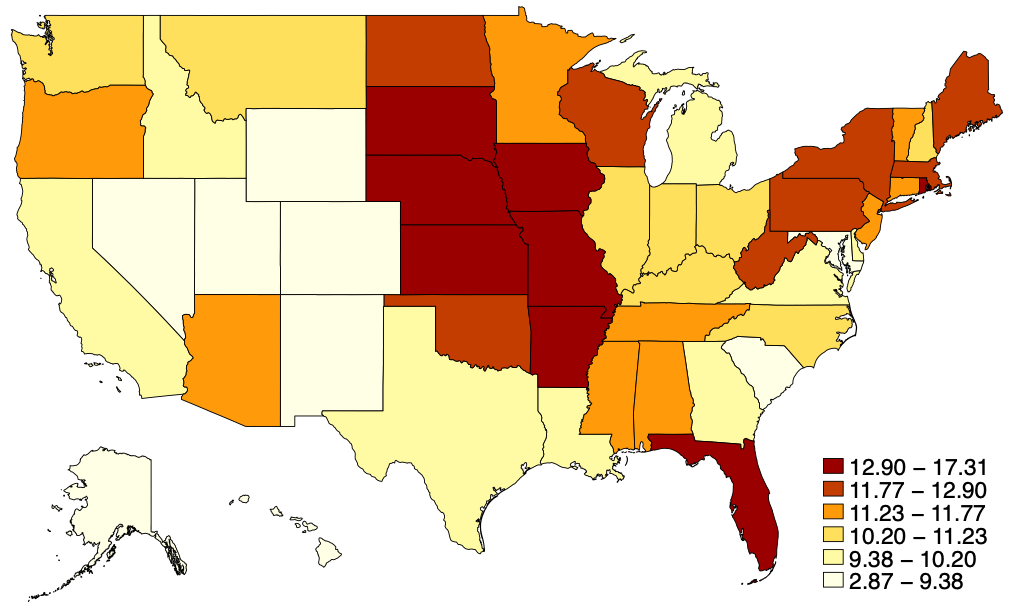
\includegraphics[width=0.49\textwidth]{Output/Figures/map1.png}} 
        \subfigure[Hexagon]{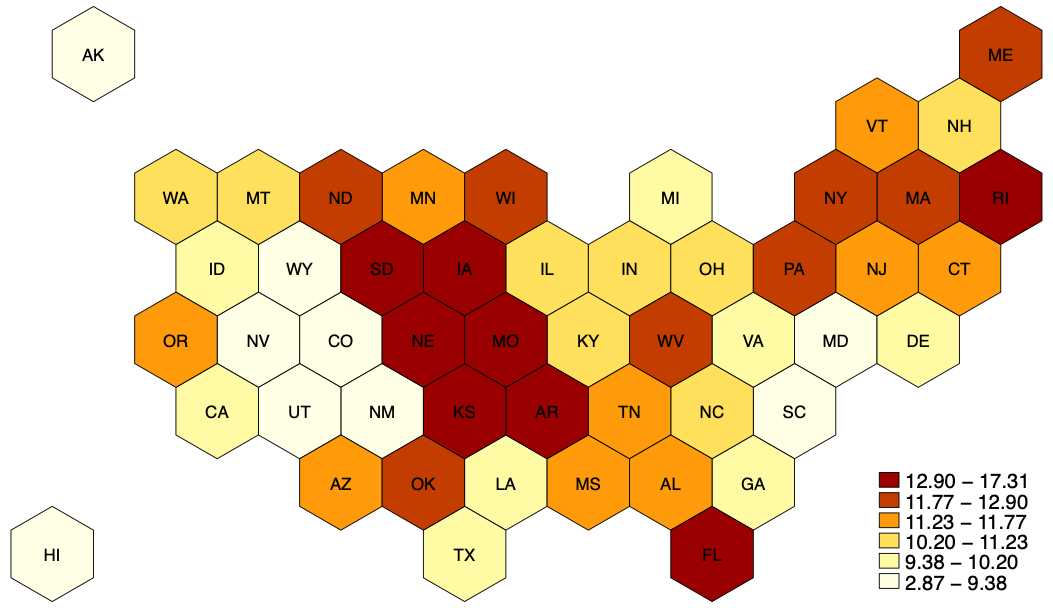
\includegraphics[width=0.49\textwidth]{Output/Figures/map2.png}} 
    \end{center}
\end{figure}

\begin{figure}[H]
    \caption{Scatter Plot}
    %\label{fig:enter-label}
    \begin{center}
        \subfigure[Version 1: Customized Markers]{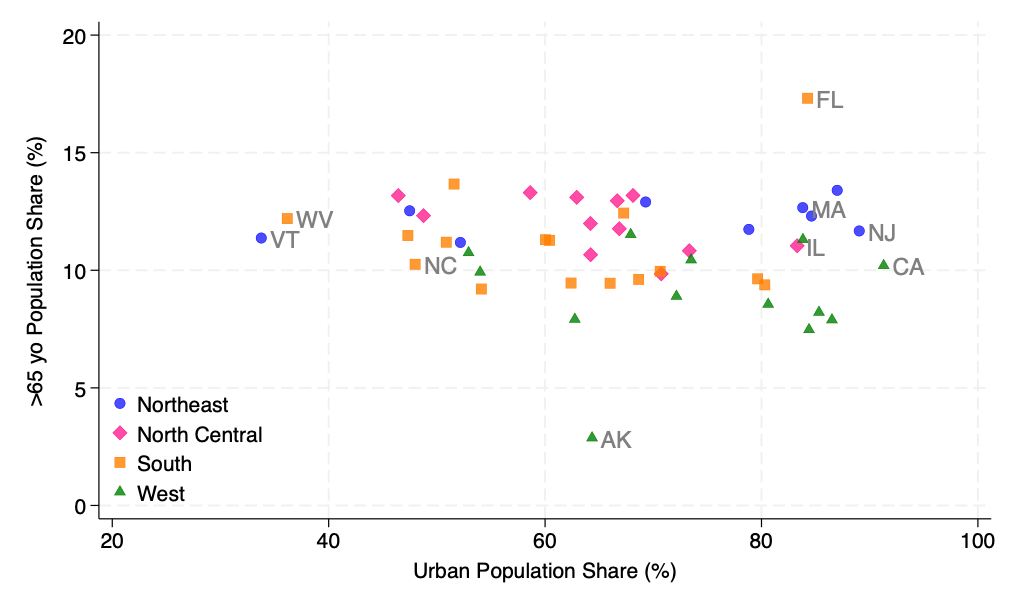
\includegraphics[width=0.49\textwidth]{Output/Figures/scatter1.png}} 
        \subfigure[Version 2: Marker Size Depends on Total Population]{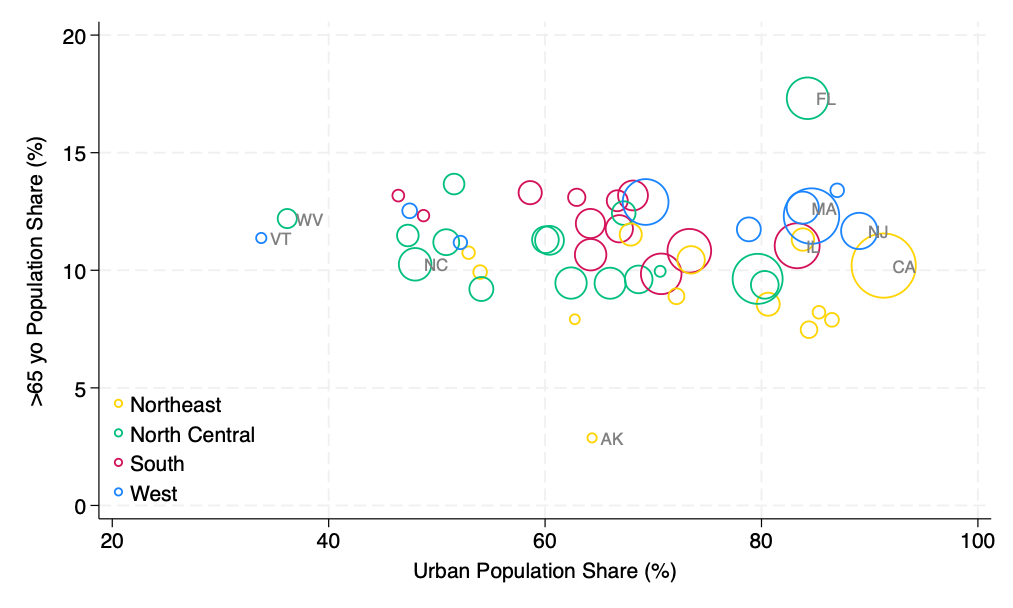
\includegraphics[width=0.49\textwidth]{Output/Figures/scatter2.png}} 
    \end{center}
\end{figure}

\begin{figure}[H]
    \centering
    \caption{A Confusing and Over-complicated Line Plot that One Should Never Put in the Paper but Just Want to Show You It's Possible}
    %\label{fig:enter-label}
    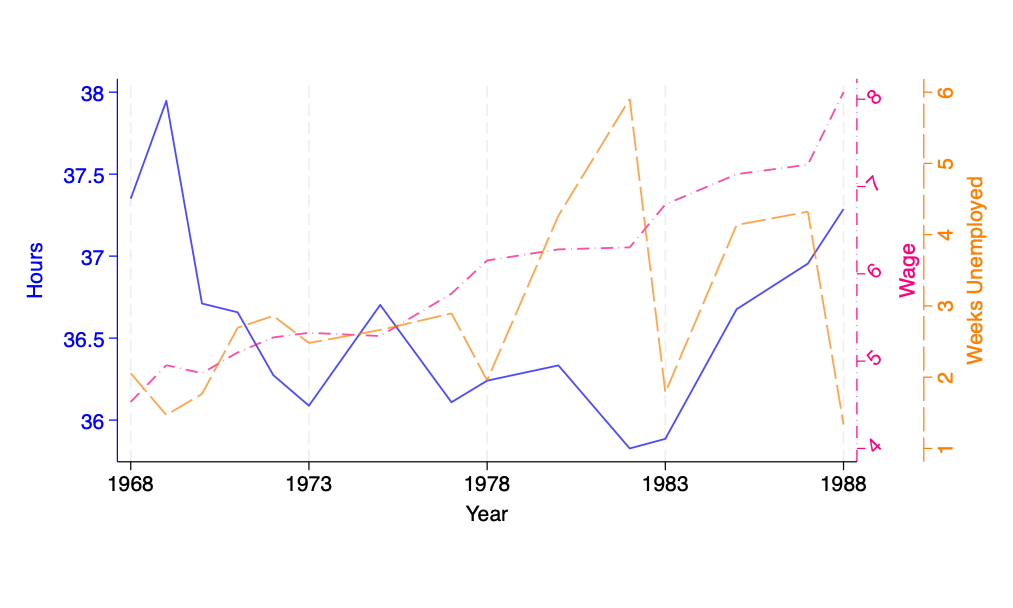
\includegraphics[width=0.9\linewidth]{Output/Figures/line.png}
\end{figure}

\begin{table}[H]
    \caption{Regression Table}
   % \label{tab:}
    \caption*{\scriptsize\textbf{Dependent Variable:} Log wage }
    \centering
    \resizebox{0.6\textwidth}{!}{ % Adjust the width of the table.
    {
\def\sym#1{\ifmmode^{#1}\else\(^{#1}\)\fi}
\begin{tabular}{l*{5}{c}}
\hline\hline
                    &\multicolumn{2}{c}{Without Fixed Effects}  &\multicolumn{3}{c}{With Fixed Effects}                           \\\cmidrule(lr){2-3}\cmidrule(lr){4-6}
                    &\multicolumn{1}{c}{(1)}         &\multicolumn{1}{c}{(2)}         &\multicolumn{1}{c}{(3)}         &\multicolumn{1}{c}{(4)}         &\multicolumn{1}{c}{(5)}         \\
\hline
In Union            &       0.224\sym{***}&       0.186\sym{***}&       0.185\sym{***}&       0.105\sym{***}&      0.0889\sym{***}\\
                    &    (0.0133)         &    (0.0128)         &    (0.0128)         &    (0.0098)         &    (0.0092)         \\
[1em]
\emph{Controls}     &                     &                     &                     &                     &                     \\
[1em]
Married             &                     &     0.00283         &     0.00422         &    -0.00692         &    -0.00551         \\
                    &                     &    (0.0118)         &    (0.0119)         &    (0.0082)         &    (0.0079)         \\
[1em]
Age                 &                     &      0.0133\sym{***}&     0.00886\sym{***}&      0.0277\sym{**} &      0.0257\sym{**} \\
                    &                     &    (0.0007)         &    (0.0022)         &    (0.0115)         &    (0.0114)         \\
[1em]
In City             &                     &      0.0651\sym{***}&      0.0652\sym{***}&      0.0231\sym{*}  &      0.0224\sym{*}  \\
                    &                     &    (0.0125)         &    (0.0125)         &    (0.0126)         &    (0.0123)         \\
[1em]
In South            &                     &      -0.186\sym{***}&      -0.185\sym{***}&     -0.0758\sym{***}&     -0.0767\sym{***}\\
                    &                     &    (0.0130)         &    (0.0130)         &    (0.0230)         &    (0.0224)         \\
[1em]
Constant            &       1.702\sym{***}&       1.347\sym{***}&       1.485\sym{***}&       0.892\sym{**} &       0.886\sym{**} \\
                    &    (0.0077)         &    (0.0238)         &    (0.0685)         &    (0.3610)         &    (0.3597)         \\
[1em]
Occupation FE       &                     &                     &                     &                     &         Yes         \\
\hline
Observations        &      19,238         &      19,215         &      19,215         &      18,548         &      18,465         \\
Dep Var Mean        &         1.8         &         1.8         &         1.8         &         1.8         &         1.8         \\
Year FE             &                     &                     &         Yes         &         Yes         &         Yes         \\
Individual FE       &                     &                     &                     &         Yes         &         Yes         \\
\hline\hline
\multicolumn{6}{l}{\footnotesize Standard errors in parentheses}\\
\multicolumn{6}{l}{\footnotesize \sym{*} \(p<0.1\), \sym{**} \(p<0.05\), \sym{***} \(p<0.01\)}\\
\end{tabular}
}

    }
    %\caption*{\scriptsize\textbf{Note:} }
\end{table}

Below is a simple demo of the \verb|xtevent| command for conducting event studies \citep{carreto2024xtevent,freyaldenhoven2021visualization}. 

\begin{figure}[H]
    \caption{Event Study using xtevent: How Union Affects Log Wage}
    %\label{fig:enter-label}
    \begin{center}
        \subfigure[TWFE]{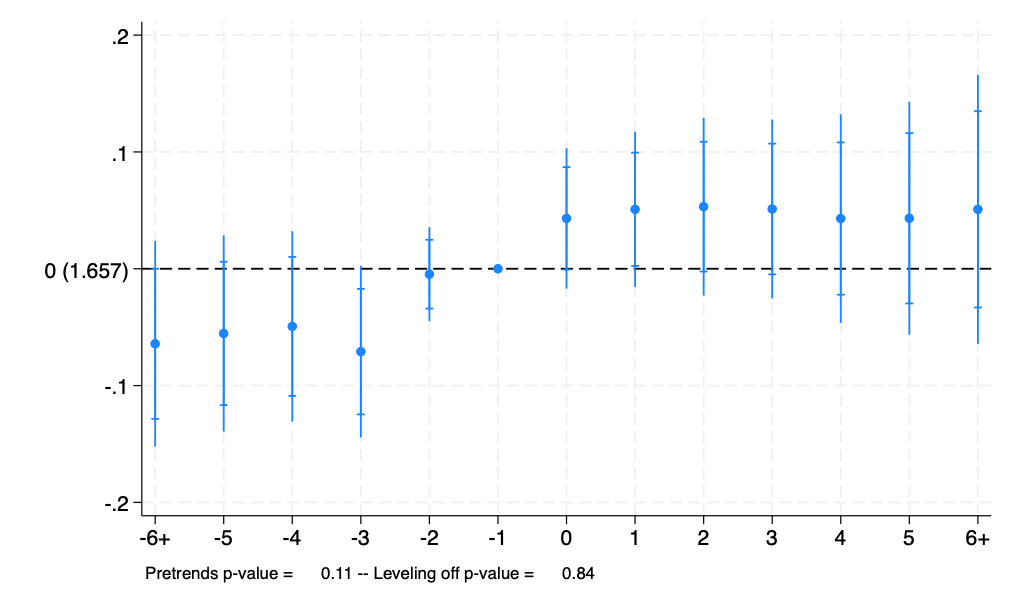
\includegraphics[width=0.49\textwidth]{Output/Figures/xtevent1.png}} 
        \subfigure[Sun and Abraham (2021)]{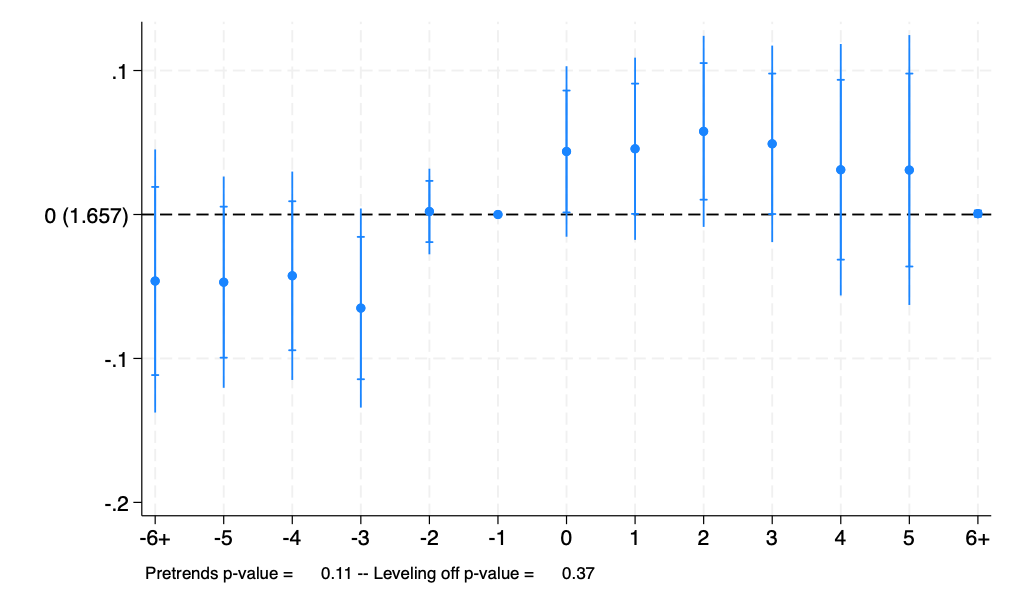
\includegraphics[width=0.49\textwidth]{Output/Figures/xtevent2.png}} 
    \end{center}
\end{figure}
